\documentclass{article}
\usepackage[backend=biber,natbib=true,style=alphabetic,maxbibnames=50]{biblatex}
\addbibresource{/home/nqbh/reference/bib.bib}
\usepackage[utf8]{vietnam}
\usepackage{tocloft}
\renewcommand{\cftsecleader}{\cftdotfill{\cftdotsep}}
\usepackage[colorlinks=true,linkcolor=blue,urlcolor=red,citecolor=magenta]{hyperref}
\usepackage{amsmath,amssymb,amsthm,enumitem,float,graphicx,mathtools,tikz}
\usetikzlibrary{angles,calc,intersections,matrix,patterns,quotes,shadings}
\allowdisplaybreaks
\newtheorem{assumption}{Assumption}
\newtheorem{baitoan}{Bài toán}
\newtheorem{cauhoi}{Câu hỏi}
\newtheorem{conjecture}{Conjecture}
\newtheorem{corollary}{Corollary}
\newtheorem{dangtoan}{Dạng toán}
\newtheorem{definition}{Definition}
\newtheorem{dinhly}{Định lý}
\newtheorem{dinhnghia}{Định nghĩa}
\newtheorem{example}{Example}
\newtheorem{ghichu}{Ghi chú}
\newtheorem{hequa}{Hệ quả}
\newtheorem{hypothesis}{Hypothesis}
\newtheorem{lemma}{Lemma}
\newtheorem{luuy}{Lưu ý}
\newtheorem{nhanxet}{Nhận xét}
\newtheorem{notation}{Notation}
\newtheorem{note}{Note}
\newtheorem{principle}{Principle}
\newtheorem{problem}{Problem}
\newtheorem{proposition}{Proposition}
\newtheorem{question}{Question}
\newtheorem{remark}{Remark}
\newtheorem{theorem}{Theorem}
\newtheorem{vidu}{Ví dụ}
\usepackage[left=1cm,right=1cm,top=5mm,bottom=5mm,footskip=4mm]{geometry}
\def\labelitemii{$\circ$}
\DeclareRobustCommand{\divby}{%
	\mathrel{\vbox{\baselineskip.65ex\lineskiplimit0pt\hbox{.}\hbox{.}\hbox{.}}}%
}
\setlist[itemize]{leftmargin=*}
\setlist[enumerate]{leftmargin=*}

\title{Lecture Note: Mathematics for Machine Learning}
\author{Nguyễn Quản Bá Hồng\footnote{A Scientist {\it\&} Creative Artist Wannabe. E-mail: {\tt nguyenquanbahong@gmail.com}. Bến Tre City, Việt Nam.}}
\date{\today}

\begin{document}
\maketitle
\begin{abstract}
	This text is a part of the series {\it Some Topics in Advanced STEM \& Beyond}:
	
	{\sc url}: \url{https://nqbh.github.io/advanced_STEM/}.
	
	Latest version:
	\begin{itemize}
		\item {\it Lecture Note: Mathematics for Machine Learning}.
		
		PDF: {\sc url}: \url{https://github.com/NQBH/advanced_STEM_beyond/blob/main/machine_learning/lecture/NQBH_mathematics_for_machine_learning_lecture.pdf}.
		
		\TeX: {\sc url}: \url{https://github.com/NQBH/advanced_STEM_beyond/blob/main/machine_learning/lecture/NQBH_mathematics_for_machine_learning_lecture.tex}.
		\item {\it Slide: Mathematics for Machine Learning -- Toán Học cho Học Máy}.
		
		PDF: {\sc url}: \url{https://github.com/NQBH/advanced_STEM_beyond/blob/main/machine_learning/slide/NQBH_mathematics_for_machine_learning_slide.pdf}.
		
		\TeX: {\sc url}: \url{https://github.com/NQBH/advanced_STEM_beyond/blob/main/machine_learning/slide/NQBH_mathematics_for_machine_learning_slide.tex}.
		\item {\it Personal Expository Notes on Machine Learning}.
		
		PDF: {\sc url}: \url{https://github.com/NQBH/draft/blob/master/machine_learning/NQBH_machine_learning.pdf}.
		
		\TeX: {\sc url}: \url{https://github.com/NQBH/draft/blob/master/machine_learning/NQBH_machine_learning.tex}.
		\item Codes:
		\begin{itemize}
			\item Python for Machine Learning: \url{https://github.com/NQBH/advanced_STEM_beyond/tree/main/machine_learning/Python}.
			\item C{\tt/}C++ for Machine Learning:
		\end{itemize}
	\end{itemize}
\end{abstract}
\tableofcontents

%------------------------------------------------------------------------------%

\begin{figure}[H]
	\centering
	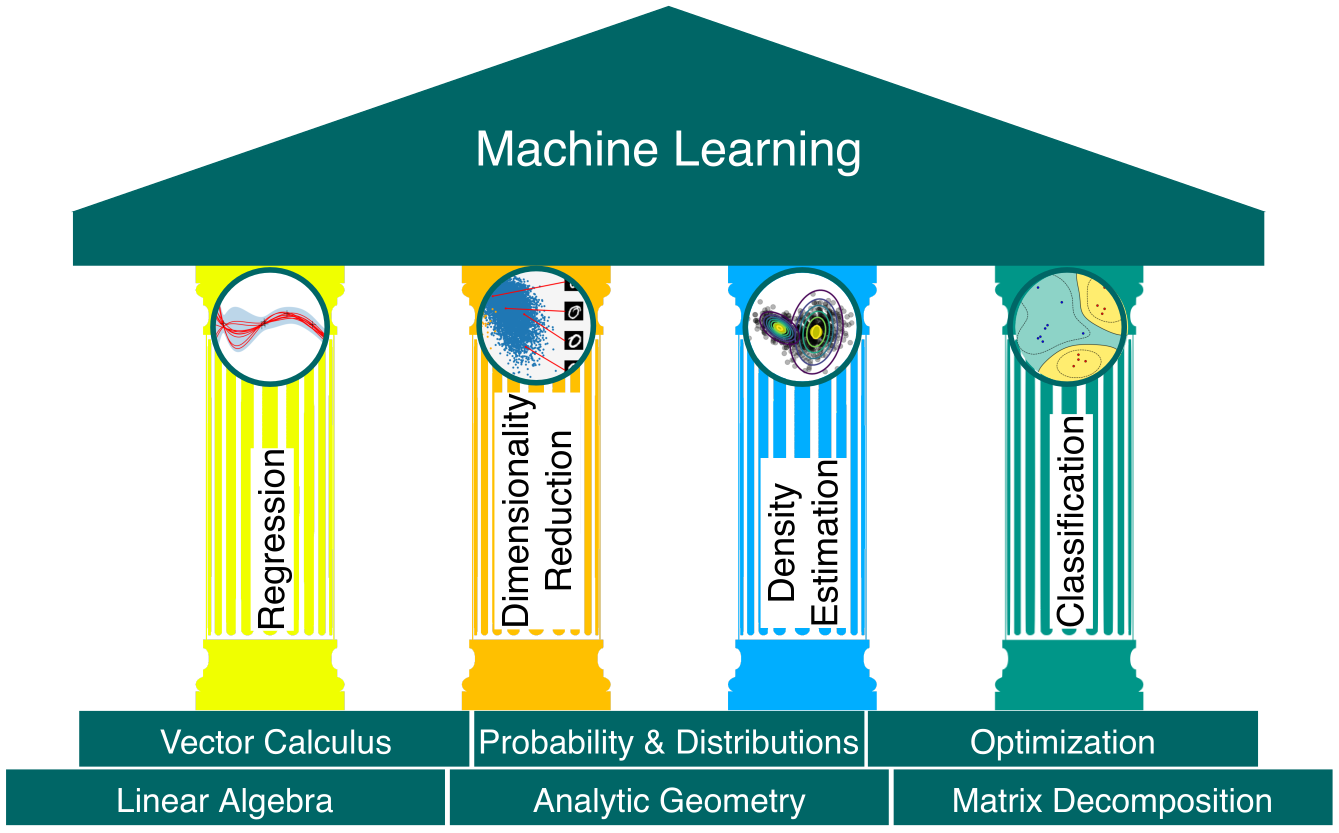
\includegraphics[width=12cm]{4_ML_pillars}
	\caption{Foundations \& 4 pillars of ML. Source: \cite[Fig. 1.1, p. 14]{Deisenroth_Faisal_Ong2023}.}
\end{figure}

\section{Linear Regression -- Hồi Quy Tuyến Tính}
\textbf{\textsf{References -- Tài nguyên.}}
\begin{enumerate}
	\item \cite{Bach2024}. {\sc Francis Bach}. {\it Learning Theory from First Principles}. Chap. 3: Linear Least-Squares Regression.
	\item \cite{Deisenroth_Faisal_Ong2023}. {\sc Marc Peter Deisenroth, A. Aldo Faisal, Cheng Soon Ong}. {\it Mathematics for Machine Learning}. Chap. 9: Linear Regression.
	\item {\sc Andrew Ng}'s Machine Learning Specialization slides: \url{}.
	\item \cite{Tiep_ML_co_ban}. {\sc Vũ Hữu Tiệp}. {\it Machine Learning Cơ Bản}. Chap. 7: Hồi Quy Tuyến Tính.
	\item Wikipedia: \href{https://en.wikipedia.org/wiki/Linear_function}{Wikipedia{\tt/}linear function}. \href{https://en.wikipedia.org/wiki/Linear_regression}{Wikipedia{\tt/}linear regression}.
\end{enumerate}
{\sf A general idea -- 1 ý tưởng tổng quát.} Ý tưởng này có vẻ được mượn từ Lý Thuyết Thống Kê Có Tham Số (Parametric Statistics Theory), see, e.g., \href{https://en.wikipedia.org/wiki/Parametric_statistics}{Wikipedia{\tt/}parametric statistics}.

For $d\in\mathbb{N}^\star$ pairs $({\bf x}_i,y_i)_{i=1}^d$ of input-output, we represent some (mathematically reasonable) hypotheses $h$ about the data using the parameters $\boldsymbol{\theta} = (\theta_1,\theta_2,\ldots,\theta_{\rm p})$ where ${\rm p} = \operatorname{size}\boldsymbol{\theta}$ is the size{\tt/}dimension (kích thước{\tt/}số chiều) of the vector of parameters, i.e., the total number of parameters in the chosen hypotheses $h$. If the data is correctly predicted according to hypothesis $h_{\boldsymbol{\theta}}$, then $y\approx h_{\boldsymbol{\theta}}({\bf x})$.

\begin{example}[Some examples of hypothesis function $h_{\boldsymbol{\theta}}$ -- Vài ví dụ về hàm giả thiết $h_{\boldsymbol{\theta}}$]
	\item(i) {\rm(Simplest: Linear function{\tt/}affine mapping)} We assume $h_{\boldsymbol{\theta}}$ be a linear function, i.e., $h_{\boldsymbol{\theta}}(x) = \theta_0 + \theta_1x$ for $d = 1$ \& $h_{\boldsymbol{\theta}}({\bf x}) = \theta_0 + [\theta_1,\theta_2,\ldots,\theta_d]\cdot{\bf x}$ for $d\ge2$.
	\item(ii) {\rm(Polynomial)}: When $d = 1$, we can assume $h_{\boldsymbol{\theta}}\in\mathbb{R}[{\bf x}]$ or even $h_{\boldsymbol{\theta}}\in\mathbb{C}[{\bf x}]$, i.e., a polynomial with real{\tt/}complex coefficients in the variable $x$:
	\begin{equation*}
		h_{\boldsymbol{\theta}}(x) = \sum_{i=0}^{\rm p} \theta_ix^i = \theta_0 + \theta_1x + \theta_2x^2 + \cdots + \theta_{\rm p}x^{\rm p}.
	\end{equation*}
	\item(iii) {\rm(Hàm phân thức)} When $d = 1$, we can assume
	\begin{equation*}
		h_{\boldsymbol{\theta}}(x) = \frac{\sum_{i=0}^m \theta_ix^i}{\sum_{m+1}^{\rm p} \theta_ix^{i-m-1}} = \frac{\theta_0 + \theta_1x + \theta_2x^2 + \cdots + \theta_mx^m}{\theta_{m+1} + \theta_{m+2}x + \cdots + \theta_{\rm p}x^{p - m - 1}}.
	\end{equation*}
	\item(iv) {\rm(Hàm căn thức)} We can assume
	\begin{align*}
		h_{\boldsymbol{\theta}}(x) &= \sqrt[n]{\sum_{i=0}^{\rm p} \theta_ix^i} = \sqrt[n]{\theta_0 + \theta_1x + \theta_2x^2 + \cdots + \theta_{\rm p}x^{\rm p}},\\
		h_{\boldsymbol{\theta}}(x) &= \sqrt[n]{\frac{\sum_{i=0}^m \theta_ix^i}{\sum_{m+1}^{\rm p} \theta_ix^{i-m-1}}} = \sqrt[n]{\frac{\theta_0 + \theta_1x + \theta_2x^2 + \cdots + \theta_mx^m}{\theta_{m+1} + \theta_{m+2}x + \cdots + \theta_{\rm p}x^{{\rm p} - m - 1}}},
	\end{align*}
	for a given (fixed) $n\in\mathbb{R}$ or an adjustable $n$, i.e., $n$ itself is also a component of $\boldsymbol{\theta}$.
	\item(v) {\rm(Elementary function -- Hàm sơ cấp)} We can assume $h_{\boldsymbol{\theta}}({\bf x})$ to be an elementary function of the variable ${\bf x}$. For elementary functions, see, e.g., \href{https://en.wikipedia.org/wiki/Elementary_function}{Wikipedia{\tt/}elementary function}.
\end{example}
A typical learning algorithm finds the best hypothesis $h_{\boldsymbol{\theta}}$ for the training set $({\bf x}_i,y_i)_{i=1}^N$. We can then estimate the values of $y$ for the test set $({\bf x}_i,y_i)_{i=N+1}^d$ using the ``optimal'' hypothesis $h_{\boldsymbol{\theta}}({\bf x})$ obtained from our learning algorithm. In particular, if $h_{\boldsymbol{\theta}}$ is a linear function of $x\in\mathbb{R}$, this procedure is called {\it linear regression}.

\subsection{Introduction to linear regression -- Giới thiệu về hồi quy tuyến tính}
{\it1st impression.} Hồi quy tuyến tính (linear regression) là:
\begin{itemize}
	\item 1 thuật toán hồi quy mà đầu ra là 1 hàm số tuyến tính (linear function, i.e., $y = ax + b$, $a,b\in\mathbb{R}$, $a\ne0$) của đầu vào. A brief notation:
	\begin{equation*}
		{\rm output} = \left\{\begin{split}
			&{\tt linear\_function}({\rm input}) = a\,{\rm input} + b&&\mbox{if } d = 1,\\
			&{\tt linear\_function}({\bf inputs}) = {\bf w}\cdot{\bf inputs} + b&&\mbox{if } d\ge2,\\
		\end{split}\right.
	\end{equation*}
	\item Thuật toán đơn giản nhất trong nhóm các thuật toán học có giám sát (supervised learning algorithms).
\end{itemize}

\begin{problem}[Housing prices -- giá cả nhà đất{\tt/}bất động sản]
	Let $m\in\mathbb{N}^\star$. Suppose we have a 2-column table whose the 1st column consists of sizes of $m$ houses: ${\bf x} = (x_1,x_2,\ldots,x_m)$ \& the 2nd one consists of their corresponding housing prices ${\bf y} = (y_1,y_2,\ldots,y_m)$. Here $m$ is the number of training examples, ${\bf x}$ is the vector of input variable or features (size), \& ${\bf y}$ is the vector of output variables or target variables (price).
\end{problem}

\begin{baitoan}[Housing price estimation -- Ước lượng giá nhà, \cite{Tiep_ML_co_ban}, Sect. 7.1, p. 100]
	Xét bài toán ước lượng giá của 1 căn phòng rộng $x_1\ {\rm m}^2$, có $x_2$ phòng ngủ, \& cách trung tâm thành phố $x_3$ km. Giả sử có 1 tập dữ diệu của $N = 10000$ căn nhà trong thành phố đó. Liệu có thể dự đoán được giá $y$ của 1 căn nhà mới (i.e., khác $N$ căn nhà đã có dữ liệu) thông qua 3 thông số về diện tích $x_1\in(0,\infty)$, số phòng ngủ $x_2\in\mathbb{N}$, \& khoảng cách tới trung tâm thành phố $x_3\in[0,\infty)$?
\end{baitoan}
{\sf Mathematical notations -- Ký hiệu toán học.} Đặt ${\bf x} = [x_1,x_2,x_3]^\top\in(0,\infty)\times\mathbb{N}\times[0,\infty)$ là 1 vector cột chứa dữ liệu đầu vào (inputs) gồm 3 thông số diện tích $x_1$, số phòng ngủ $x_2$, \& khoảng cách đến trung tâm thành phố $x_3$; ${\bf x}$ được gọi là {\it vector đặc trưng}. Đặt giá nhà (đầu ra{\tt/}output) $y\in(0,\infty)$.

{\sf Reasoning -- Biện luận.} Nếu diện tích nhà càng lớn thì giá nhà càng cao: $x_1\uparrow\Rightarrow y\uparrow$, nếu nhà có càng nhiều phòng ngủ thì giá nhà càng cao: $x_2\uparrow\Rightarrow y\uparrow$, \& nếu nhà càng ở gần trung tâm thành phố thì giá nhà càng cao: $x_3\downarrow0\Rightarrow y\uparrow$ (why? economics!). Có thể sử dụng mô hình đầu ra là 1 hàm tuyến tính đơn giản của đầu vào:
\begin{equation}
	\label{linear relation}
	\tag{lnr}
	y\approx\hat{y}\coloneqq f({\bf x}) = w_1x_1 + w_2x_2 + w_3x_3 = \sum_{i=1}^3 w_ix_i = {\bf x}^\top{\bf w} = {\bf w}^\top{\bf x} = {\bf x}\cdot{\bf w} = \langle{\bf x},{\bf w}\rangle,
\end{equation}
với ${\bf w} = [w_1,w_2,w_2]^\top$ là {\it vector trọng số} (weight vector) với $w_1,w_2\in(0,\infty),w_3\in(-\infty,0)$ (why?) cần tìm. Mối quan hệ cho bởi \eqref{linear relation} là 1 mối quan hệ tuyến tính.

\begin{question}[Regression factor]
	Why is it called \emph{regression}?
\end{question}
{\it Bản chất.} 2 bài toán dự đoán giá nhà trên là 2 bài toán dự đoán giá trị đầu ra dưa trên vector đặc trưng đầu vào. Ngoài ra, giá trị của đầu ra $y$ có thể nhận rất nhiều giá trị thực dương khác nhau. Nên ta cần tính đi tính lại, tính kết quả đầu ra mới dựa trên các kết quả đầu ra cũ, để nhận được 1 kết quả được xem là tối ưu theo nghĩa nào đó. Vì vậy, đây cũng là 1 bài toán hồi quy. Kết hợp bản chất hồi quy với mối quan hê tuyến tính $\hat{y} = {\bf x}^\top{\bf w}$ cho ra tên gọi {\it hồi quy tuyến tính}. Về hàm tuyến tính, see, e.g., \href{https://en.wikipedia.org/wiki/Linear_function}{Wikipedia{\tt/}linear function}.

{\sf Some reasons to study linear least-squares regression.} From \cite[Sect. 3.1, pp. 45--46]{Bach2024}.
\begin{itemize}
	\item Linear least-squares regression already captures many of the concepts in learning theory, e.g. bias-variance trade-off, as well as dependence of generalization performance on the underlying dimension of the problem with no regularization, or on dimensionless quantities when regularization is added.
	
	-- Hồi quy tuyến tính bình phương nhỏ nhất đã nắm bắt được nhiều khái niệm trong lý thuyết học tập, ví dụ như sự đánh đổi giữa độ lệch và phương sai, cũng như sự phụ thuộc của hiệu suất tổng quát vào chiều cơ bản của vấn đề không có chính quy hóa hoặc vào các đại lượng không có thứ nguyên khi chính quy hóa được thêm vào.
	\item Because of its simplicity, many results can be easily derived without the need for complicated mathematics, both in terms of algorithms \& statistical analysis (simple linear algebra for the simplest results in the fixed design setting).
	
	-- Do tính đơn giản của nó, nhiều kết quả có thể dễ dàng thu được mà không cần đến các phép toán phức tạp, cả về mặt thuật toán \& phân tích thống kê (đại số tuyến tính đơn giản cho kết quả đơn giản nhất trong bối cảnh thiết kế cố định).
	\item Using nonlinear features, it can lead to arbitrary nonlinear predictions.
	
	-- Sử dụng các tính năng phi tuyến tính, nó có thể dẫn đến những dự đoán phi tuyến tính tùy ý.
\end{itemize}

\begin{question}[Optimal choice of parameters $\boldsymbol{\theta}$]
	How to choose parameters $\boldsymbol{\theta}$ ``optimally''? ``Optimal'' in which sense?
	
	-- Làm thế nào để chọn tham số $\boldsymbol{\theta}$ ``tối ưu''? ``Tối ưu'' theo nghĩa nào?
\end{question}

\subsection{A general mathematical setting}
Tổng quát, nếu mỗi điểm dữ liệu được mô tả bởi 1 vector đặc trưng $d$ chiều $x\in\mathbb{R}^d$, hàm dự đoán đầu ra được viết dưới dạng
\begin{equation*}
	y = {\bf x}^\top{\bf w} = {\bf x}\cdot{\bf w} = \sum_{i=1}^d w_ix_i = w_1x_1 + \cdots + w_dx_d.
\end{equation*}
Nếu tính thêm bias (e.g., tiện đặt cọc, chi phí phát sinh, giảm giá, voucher discount, etc.) $b\in\mathbb{R}$ thì thêm vào thành:
\begin{equation*}
	y = {\bf x}^\top{\bf w} + b = {\bf x}\cdot{\bf w} + b = \sum_{i=1}^d w_ix_i + b = w_1x_1 + \cdots + w_dx_d + b.
\end{equation*}

Với bài toán hồi quy nói chung, ta cần cực tiểu sự sai khác $e$ (error) giữa đầu ra thực sự $y$ \& đầu ra dự đoán $\hat{y}$ với $e$ thường được chọn khoảng cách giữa 2 điểm $y$ \& $\hat{y}$, e.g.:
\begin{equation*}
	\frac{1}{2}e^2 = \frac{1}{2}(y - \hat{y})^2 = \frac{1}{2}(y - {\bf x}^\top{\bf w} - b)^2.
\end{equation*}
(Hệ số $\frac{1}{2}$ đóng vai trò là scaling factor, giúp khi tính đạo hàm thì sẽ đơn giản được hệ số, thật vậy: vì $\left(\frac{1}{2}x^2\right)' = x$ nên hệ số $\frac{1}{2}$ sẽ bị triệ tiêu khi lấy đạo hàm của $e$ theo tham số mô hình ${\bf w}$.) Các cách chọn sai số $e$ khác:
\begin{enumerate}
	\item $e = y - \hat{y}$: Khuyết điểm: $y - \hat{y}$ có thể âm, do đó việc cực tiểu hóa $e$ không có ý nghĩa.
	\item $e = |y - \hat{y}|$: Khuyết điểm: Hàm trị tuyệt đối (absolute value function) $f:\mathbb{R}\to[0,\infty)$, $f(x) = |x|$ tuy liên tục nhưng không khả vi tại gốc tọa độ (why?), không thuận tiện cho việc tối ưu.
	\item $e = \frac{1}{p}|y - \hat{y}|^p$ với $p\in(1,\infty)$. Hàm số $f(x) = \frac{1}{p}x^p$ có đạo hàm $f'(x) =|x|^{p-1}$. Khuyết điểm: Cần nhiều tính toán hơn số với hàm bình phương, i.e., khi $p = 2$.
\end{enumerate}

Hàm mất mát đóng vai trò là tiêu chí cho việc tối ưu mô hình: việc tìm mô hình tốt nhất{\tt/}tối ưu nhất (best{\tt/}optimal) tương đương với việc tìm ${\bf w}$ để cực tiểu hàm số:
\begin{equation*}
	L({\bf w}) = \frac{1}{2N}\sum_{i=1}^N (y_i - {\bf x}_i^\top{\bf w})^2.
\end{equation*}
Optimization problem -- Bài toán tối ưu:
\begin{equation*}
	\min_{\bf w} L({\bf w}).
\end{equation*}
Nếu bài toán có nghiệm duy nhất, ký hiệu:
\begin{equation*}
	{\bf w}^* = {\arg\min}_{\bf w} L({\bf w}).
\end{equation*}

%------------------------------------------------------------------------------%

\section{Overfitting -- Quá Khớp}

%------------------------------------------------------------------------------%

\section{$K$ Neighbors -- $K$ Lân Cận}

%------------------------------------------------------------------------------%

\section{Phân Cụm $K$-Means}

%------------------------------------------------------------------------------%

\section{Artificial Neural Networks (ANNs) -- Mạng Neuron Nhân Tạo}

Distinguish: Artificial Neural Network (ANN) vs. Biological Neural Network (BNN), see, e.g., \href{https://en.wikipedia.org/wiki/Neural_network_(machine_learning)}{Wikipedia{\tt/}neural network (machine learning)} vs. \href{https://en.wikipedia.org/wiki/Neural_network_(biology)}{Wikipedia{\tt/}neural network (biology)}, \href{https://psychology.fandom.com/wiki/Biological_neural_networks}{Psychology Wiki{\tt/}biological neural network}.

\begin{definition}[Activation function $\sigma(\cdot)$]
	
\end{definition}

\begin{figure}[H]
	\centering
	
\includegraphics[height=6cm]{neuron_activation_anime}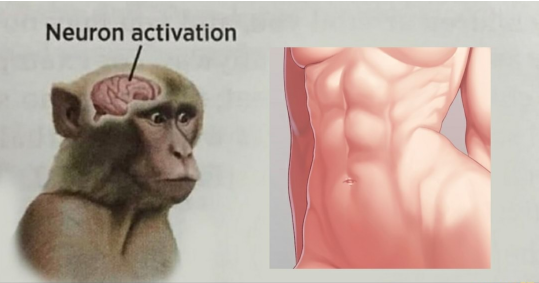
\includegraphics[height=6cm]{neuron_activation}
	\caption{A typical monkey's (maybe man also?) biological neural networks (BNN) gets activated by 2D{\tt/}anime girl's strong abs.}
\end{figure}

%------------------------------------------------------------------------------%

\section{Perception Learning Algorithm -- Thuật Toán Học Perceptron}

%------------------------------------------------------------------------------%

\section{Logistic Regression -- Hồi Quy Logistic}

%------------------------------------------------------------------------------%

\section{Softmax Regression -- Hồi Quy Softmax}

%------------------------------------------------------------------------------%

\section{Deep Neural Networks \& Backpropagation -- Mạng Neuron Đa Tầng \& Lan Truyền Ngược}

%------------------------------------------------------------------------------%

\section{Miscellaneous}

\subsection{Contributors}

%------------------------------------------------------------------------------%

\printbibliography[heading=bibintoc]
	
\end{document}